To begin with, this chapter will give an overview of the general purpose, the contained components and the fundamental functionality of a blockchain. 

\subsection{General Purpose}
In general, a blockchain can be described as a digital data structure that can be understand as a shared and distributed database, containing a continuous expanding and chronological log of transactions \cite{andoni2019blockchain}. Besides, various types like digital transactions, data records and executables can be stored in this digital data structure. The data transmission in a blockchain is comparable with copying data from one computer to another. However, the resulting challenge is that the system needs to ensure that the data is copied just once \cite{andoni2019blockchain}. For example, in the domain of cryptocurrencies, this is equal to sending a coin from one wallet to another. In this case, the system needs to validate that this coin is spended just once and there is no double-spending. A conventional solution for this problem is a third intermediary. To come back to the stated example, the third intermediary is represented by a traditional bank, which store, protect and continuously update the valid state of the ledger \cite{andoni2019blockchain}. But, in some cases central management is not practicable or reasonable. Reasons for this are possible intermediary costs or a high degree of trust of the users into the intermediary who operates the system. Further, central management has a significant disadvantage because of a single point of failure. Hence, the centralized system is fragile to technical problems as well to external malicious attacks \cite{andoni2019blockchain}.
Consequently, the main reason of bockchain technologies is the removal of such third trusted intermediaries through a distributed network of various users, who cooperating together to verify transactions and protect the validity of the ledger

\subsection{Architecture}
This subsection covers the architectural design of a blockchain and presents all contained components in detail. Due to the plurality of the blockchain technologies, each of the technology slightly differs in design and components. The following explanations are oriented torwards the Ethereum blockchain implementation, which is also used as the underlying ICT to implement the open simulation platform.

\subsubsection{World State}
\label{sec:world_state}
Referring to the \textit{Yellow Paper} \cite{wood2014ethereum}, Ethereum can be seen as a transaction-based state machine. What does that mean? At the beginning, Ethereums state machine starting with a so called \textit{"genesis state"}. This is analogous to a blank sheet. On this state, no transactions have happened on the network. Next, transactions are executed and the state of the Ethereum world changes into a new state. Further, transactions are executed incrementally and morph it into some final state. Consequently, the final state is accepted as the canonical version of the world of Ethereum and represents at any times the current state.

\begin{figure}[htbp]
	\centering
	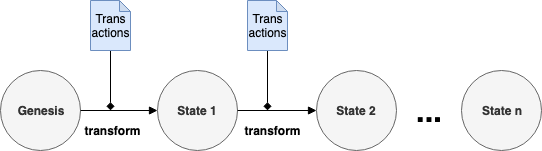
\includegraphics[width=.9\linewidth]{./figures/state_transition.png}
	\caption{World State: Transition of States}
	\label{figure:state_transition}
\end{figure}

In more detail, the world state arises out of a mapping of accounts and account states \cite{wood2014ethereum}. However, the world state is not stored on the blockchain itself. This mapping is stored and maintained in a modified data structure called a \textit{Merkle Patricia tree}. , this tree is stored off-chain (i.e. on a users computer running an Ethereum client) in a simple database backend, also known as the \textit{state database} in the Ethereum world \cite{wood2014ethereum}. To get a better understanding of the operating principles of the blockchain, it is necessary to get an idea of how a \textit{Merkle Patricia tree} works. A \textit{Merkle Patricia tree} is a type of binary tree, which consists of a set of nodes. It has a large amount of 
\textit{leaf nodes}, containing the underlying data. Further, a set of intermediate nodes, where each node is the hash of its two children, and finally, one single root node, representing the top of the tree which is also build out of its two child nodes \cite{buterin2013next} \cite{wood2014ethereum}.
As mentioned before, the \textit{leaf nodes} contain the stored data by splitting these data into chunks. Afterwards, these chunks are splitted into buckets. Then, each bucket gets hashed and the same process repeats, traversing upwards the tree, until the total number of hashes remaining becomes only one and the root node is reached. 

\begin{figure}[htbp]
	\centering
	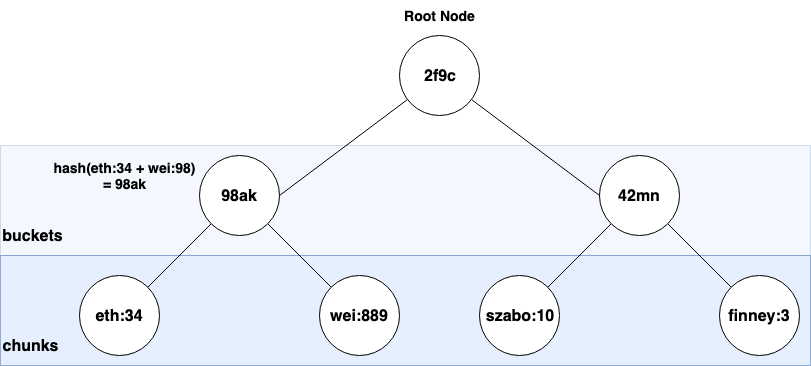
\includegraphics[width=.9\linewidth]{./figures/merkle_tree.png}
	\caption{Example of a Patricia Merkle tree}
	\label{figure:merkle_tree}
\end{figure}

Therefore, any change to the underlying data, stored in a \textit{leaf node}, causes a change of the hash of the node. Each parent's node hash depend on the data of its children. Due to this, any change to the data of a child node causes the parent hash to change. This procedure repeats traversing upwards until the root node. Hence, any change to the data at the leaf nodes effects the root hash \cite{ethereum_wiki}. 

\begin{figure}[htbp]
	\centering
	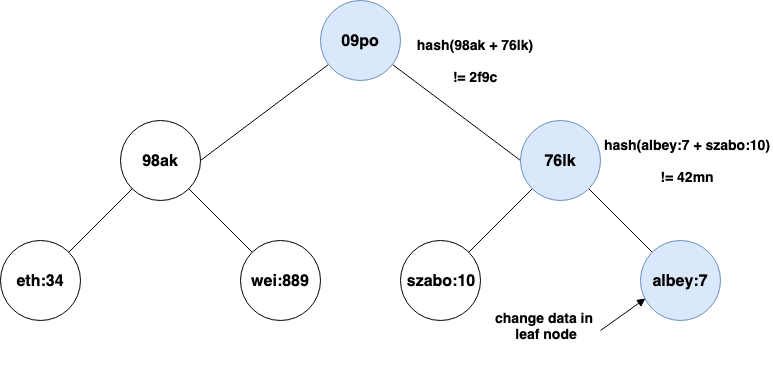
\includegraphics[width=.9\linewidth]{./figures/merkle_tree_change.png}
	\caption{Example of a data change in a leaf node}
	\label{figure:merkle_tree_change}
\end{figure}

Because of this characteristic, it is not necessary to compare the data of the entire tree. It is sufficient to compare the single root hash to ensure that all the data are the same. This property is very important, because it makes it possible to store only the hash of the root node to represent a state of the ethereum world. 


\subsubsection{Block} 
As described in \ref{sec:world_state}, whenever transactions are executed, the state of the Ethereum world changes into a new state. Every state and the belonging transactions, which transform the prior state into the new state, is stated in a so called block. That means, states are represented by blocks. As you can see in figure \ref{figure:state_transition}, the history of the Ethereum world is a linkage of states, or in other words, blocks. That is where the name blockchain comes from. A blockchain is a sequence of blocks, which holds a complete list of transaction records \cite{zheng2017overview}. 
Moreover, a block is a collection of different relevant informations and consists of the \textit{block header} and the \textit{block body}, which contains the list of transactions. Following \textit{Ethereums Yellow Paper} \cite{wood2014ethereum}, the subsequent pieces of information are contained in the \textit{block header}:

\begin{description}
	\item[Parent Hash:] This is the hash of the parents block's header
	\item[Beneficiary:] The miners address to which all block rewards from the successful mining of a block are transferred.
	\item[State Root:] This is the hash of the root node of the state tree, after a block and its transactions are finalized. As mentioned in \ref{sec:world_state}, the state tree is the one and only global state in the Ethereum world. It is used as a secure unqiue identifier for the state and the state root node is cryptographically dependent on all internal state tree data.
	\item[Transactions Root:] This is the hash of the root node of the transaction tree. This tree contains all transactions in the block body. In contrast to the state tree, there is a separate transactions tree for every block. 
	\item[Receipts Root:] Every time a transaction is executed, Ethereum generates a transaction receipt that contains information about the transaction execution. This field is the hash of the root node of the transactions receipt tree and like the transaction tree, there is a seperate receipt tree for every block.
	\item[Difficulty:] This is a measure of how hard it was to mine this block – a quantity calculated from the previous block’s difficulty and its timestamp
	\item[Number:] This is a quantity equal to the number of blocks that precede the current block in the blockchain.
	\item[Gas Limit:] This is a quantity equal to the current maximum gas expenditure per block. Each transaction consumes gas. The gas limit specifies the maximum gas that can be used by the transactions included in the block. It is a way to limit the number of transactions in a block.
	\item[Gas Used:] This is a quantity equal to the total gas used in transactions in this block.
	\item[Timestamp:] This is a record of Unix’s time at this block’s inception.
	\item[Nonce:] This is an 8-byte hash that verifies a sufficient amount of computation has been done on this block. Further, it is a number added to a hashed block that, when rehashed, meets the difficulty level restrictions. The nonce is the number that blockchain miners are solving for.
\end{description}

\subsubsection{Mining}
